\begin{theorem}[O rozvoji holomorfní funkce na kruhu do mocninné řady]
Nechť $R \in (0, +\infty]$ a $f \in \Holo (U(z_0,\,R))$. Potom existuje jediná mocninná řada $\sum\limits _{n=0} ^{\infty} a_n(z-z_0)^n$, která má na $U(z_0,\,R)$ součet $f$. Navíc platí, že $a_n=\frac{f^{(n)}(z_0)}{n!}$, $n \in \N_0$.
\end{theorem}

\begin{proof}
\begin{enumerate}
    \item jednoznačnost: Zřejmě z toho, že $a_n=\frac{f^{(n)}(z_0)}{n!}$, $n \in \N_0$.
    \item existence: Nechť $z \in U(z_0,\,R)$. Volme $r>0$, aby $|z-z_0|<r<R$. Potom z \cref{eqn:cvz} je
    \begin{equation}
        f(z)=\frac{1}{2 \pi i} \int_\varphi \frac{f(w)}{w-z} \diff w,
        \tag{a}
        \label{eqn:6.4a}
    \end{equation}
    
    kde $\varphi(t)=z_0+re^{it} \text{, } t \in [0,\,2\pi]$.
    
    Pro každé $w \in \langle \varphi \rangle$ máme
    \begin{equation}
        \quad \frac{1}{w-z}=\frac{1}{(w-z_0)-(z-z_0)}=\frac{1}{w-z_0}\cdot\frac{1}{1-\frac{z-z_0}{w-z_0}}=\sum_{n=0}^\infty \frac{(z-z_0)^n}{(w-z_0)^{n+1}} \text{.}    
        \label{eqn:6.4b}
        \tag{b}
    \end{equation}
    
    Kde $|\frac{z-z_0}{w-z_0}|<1$ a suma konverguje stejnoměrně pro $w \in  \langle \varphi \rangle$. Dosadíme \cref{eqn:6.4a} do \cref{eqn:6.4b}. Potom
    \begin{equation*}
        \begin{split}
    f(z) &=\frac{1}{2 \pi i} \int_\varphi \sum_{n=0}^\infty \frac{(z-z_0)^n}{(w-z_0)^{n+1}} f(w) \diff w= 
    \sum_{n=0}^\infty (z-z_0)^n \frac{1}{2 \pi i} \int_\varphi \frac{f(w)}{(w-z_0)^{n+1}} \diff w \\
     &=\sum_{n=0}^\infty (z-z_0)^n \frac{f^{(n)}(z_0)}{n!}
     \end{split}
    \end{equation*}
    z \cref{eqn:cvkz}.
\end{enumerate}
\end{proof}

\begin{example}
$e^z=\sum\limits_{n=0}^\infty \frac{z^n}{n!}$, $z \in \Comp  $, protože $\exp \in \Holo (\Comp  )$ a $\exp^{(n)}(0)=\exp(0)=1$.
\end{example}

\newpage
\begin{theorem}[O nulovém bodě]
Nechť $f$ je holomorfní funkce na okolí $z_0 \in \Comp  $ a $f(z_0)=0$. Potom buď
\begin{enumerate}
    \item existuje $r>0$, že $f=0$ na $U(z_0,\,r)$, nebo
    \item existuje $r>0$, že $f\neq 0$ na $P(z_0,r):=U(z_0,\,r)\backslash \{z_0\}$.
\end{enumerate}
V případě 2. existuje jediné $p\in \N$ takové, že 
\begin{equation}
    f(z_0)=f'(z_0)= \ldots = f^{(p-1)}(z_0)=0,\hspace{5mm}
    f^{(p)}(z_0) \neq 0.
    \label{eqn:6.6.0}
\end{equation}
Číslo $p$ nazýváme násobnost nulového bodu $z_0$ funkce $f$.
\end{theorem}

\begin{note}
Navíc $z_0$ je nulový bod $f$ násobnosti $p$, právě když existuje $r>0$ a $g \in \Holo (U(z_0,\,r))$ tak, že $\forall z \in U(z_0,r)$: 
\begin{equation}
    g(z) \neq 0 \hspace{3mm}\text{ a }\hspace{3mm} f(z)=(z-z_0)^p g(z).
    \label{eqn:6.7.t}
\end{equation}
\end{note}

\begin{proof}
Máme, že $f(z)=\sum\limits _{n=0} ^{\infty} a_n(z-z_0)^n$, $z \in U(z_0,\,r)$. Pokud nenastane 1., potom existuje $n \in \N$, že $0 \neq a_n=\frac{f^{(n)}(z_0)}{n!}$. Zvolme nejmenší $p \in \N$, aby $a_p \neq 0$. Potom platí \cref{eqn:6.6.0} a
\begin{equation}
    \forall z \in U(z_0,r):\ f(z)=a_p(z-z_0)^p + \ldots = (z-z_0)^p \cdot \underset{:=\ g(z)}{\underbrace{\sum\limits_{n=p}^\infty a_n(z-z_0)^{n-p}}}.
\end{equation} 
Dále $g(z)$ definujeme jako poslední sumu. %Nebo-li g(z):=\sum\limits_{n=p}^\infty a_n(z-z_0)^{n-p}$
Protože $g(z_0)=a_p \neq 0$, existuje $r>0$, že $g \neq 0$ na $U(z_0,\,r)$ a $f(z)=(z-z_0)^pg(z) \neq 0$ na $P(z_0,r)$. Obrácené tvrzení z poznámky je snadné.
\end{proof}

\begin{theorem}[O jednoznačnosti pro holomorfní funkce]\label{thm:jednoznacnostHolo}
Nechť $\emptyset \neq G \subset \Comp  $ je oblast a $f,g \in \Holo (G)$. Pak jsou následující tvrzení ekvivalentní:
\begin{enumerate}
\item $f=g$ na $G$;
\item množina $M:=\{z \in G : f(z)=g(z) \}$ má v $G$ hromadný bod, tj. existuje $z_0 \in G$ takový, že $\forall  r>0:\  M \cap P(z_0,\,r) \neq \emptyset  \;$
\item existuje $z_0 \in G$, že $\forall k \in \N_0: \ f^{(k)}(z_0)=g^{(k)}(z_0) \;$.
\end{enumerate}
\end{theorem}

\begin{proof}
Bez újmy na obecnosti $g \equiv 0$ na $G$ (jinak uvažme $f-g$).

1 $\Rightarrow$ 2: triviální, 2 $\Rightarrow$ 3: Nechť $z_0 \in G$ je hromadný bod $M:=\{z \in G :\ f(z)=0 \}$. Z věty o nulovém bodě je $f=0$ na nějakém okolí $z_0$, tudíž platí 3.

3 $\Rightarrow$ 1: Nechť $N:=\{z \in G: \ \forall k \in \N_0: f^{(k)}(z)=0 \}$. Potom $\emptyset  \neq N$, $N$ je uzavřená v $G$, protože všechny $f^{(k)}$ jsou spojité. Navíc $N$ je otevřená. Nechť $z_1 \in N$. Podle věty o nulovém bodě existuje $r>0$, že $f=0$ na $U(z_1,r)$. Tedy $U(z_1,r) \subset N$. Protože $G$ je oblast, dostaneme $N=G$ a speciálně 1.
\end{proof}

\begin{example}
Vzoreček $\sin (2z)=2\sin (z) \cos (z)$, $z \in \Comp  $ dostaneme z věty o jednoznačnosti, protože obě strany rovnosti jsou celé funkce a víme, že rovnost platí na $\Real $ (tzn. platí 2).
\end{example}

\begin{note}
Podobně lze řadu vzorečků bez počítání zobecnit z $\Real $ do $\Comp  $!
\end{note}

\begin{theorem}[Princip maxima modulu]
Nechť $G \subset \Comp  $ je oblast a $f\in \Holo (G)$. Potom je $f$ konstantní na $G$, pokud $|f|$ nabývá na $G$ lokální maximum, tzn. existuje $z_0 \in G$ a $r>0$ tak, že 
\begin{equation}
    \forall z \in U(z_0,r) \subset G:\ |f(z)| \leq |f(z_0)|
    \label{eqn:6.8.+}
\end{equation}
\end{theorem}

\begin{proof}
Nechť platí \cref{eqn:6.8.+}. Potom $f(z)=\sum\limits_{n=0}^\infty a_n(z-z_0)^{n}$, $z\in U(z_0,r)$. Pro $0<\rho<r$ platí, že 
\begin{equation}
    \begin{aligned}
    |a_0|^2 &=
    |f(z_0)|^2 \geq 
    \frac{1}{2 \pi} \int_{0}^{2 \pi} |f(z_0+\rho e^{it})|^2 \diff t =
    %tato rovnost plyne z toho,že $|f(z)|^2=f(z)\cdot \overline {f(z)}$
    \frac{1}{2\pi} \int_{0}^{2 \pi} \left(\sum\limits_{n=0}^\infty a_n \rho^n e^{int}\right)\left(\sum\limits_{m=0}^\infty \overline{a_m} \rho^m e^{-imt}\right) \diff t  \\
    %Jelikož obě řady konvergují stejnoměrně a absolutně pro $t\in[0,2\pi]$, tak i jejich součin konverguje stejnoměrně a absolutně.
    & = \sum\limits_{n=0}^\infty \sum\limits_{m=0}^\infty a_n\cdot \overline{a_m} \rho^{n+m} \frac{1}{2 \pi} \int_{0}^{2 \pi}  e^{it(n-m)} \diff t=\sum\limits_{n=0}^\infty |a_n|^2\rho^{2n},
    \end{aligned}
\end{equation}
 neboť
 $$\frac{1}{2 \pi} \int_{0}^{2 \pi}  e^{it(n-m)} \diff t = \twopartdef{0}{n \neq m,}{1}{n = m.}$$ 

Nebo-li $|a_0|^2\geq|a_0|^2+|a_1|^2\rho^2+\cdots$, tudíž $0=a_1=a_2=\cdots$. Dostáváme, že $f=a_0$ na $U(z_0,r)$ a z věty o jednoznačnosti $f=a_0$ na $G$.
\end{proof}

\section{\texorpdfstring{Riemannova sféra}{Riemannova sféra}} \setcounter{equation}{0}
Rozšíříme $\Comp  $ o \emph{nekonečno}.
Položíme $\Sp=\Comp  \cup\{\infty\}$, kde $\infty\notin\Comp  $, a pro $\varepsilon>0$ zavedeme \emph{okolí} kolem $\infty$, následovně $P(\infty,\,\varepsilon):=\{z\in\Comp  : |z|>\frac{1}{\varepsilon}\}$,
$U(\infty,\,\varepsilon):=P(\infty,\,\varepsilon)\cup \{\infty\}$.

\begin{definition}
Řekneme, že $z_n\rightarrow z_0$ v $\Sp$, pokud $\forall\varepsilon>0\textbf{ }  \exists n_0\in\N\textbf{ }\forall n\geq n_0:z_n\in U(z_0,\,\varepsilon)$.
\end{definition}

\begin{note} Z definice plyne:
\begin{itemize}
    \item $z_n\rightarrow z_0$ v $\Sp$ a $z_0\in\Comp  \Leftrightarrow z_n\rightarrow z_0$ v $\Comp  $.
    \item $z_n\rightarrow\infty\Leftrightarrow|z_n|\rightarrow+\infty\Leftrightarrow\frac{1}{z_n}\rightarrow 0$. Zde $\frac{1}{\infty}:=0$ a $|\infty|:=+\infty$.
\end{itemize}
\end{note}

\begin{note}
$\Sp$ je jednobodová kompaktifikace topologického prostoru $\Comp  $.
\end{note}

\begin{properties}%proč se Riemannově sféře říká Riemannova sféra
Na $\Sp$ zavedeme metriku $\varrho$ (není jediná), tž.
\begin{equation}
    \left( z_n\overset{n\to\infty}{\longrightarrow} z_0 \text{  v  } \Sp \right)
    \Leftrightarrow \varrho(z_n,\,z_0)\overset{n\to\infty}{\longrightarrow} 0.
    \label{eqn:7.4.*}
    \tag{*}
\end{equation} Navíc $(\Sp,\varrho)$ bude \emph{izometrický} s jednotkovou sférou $S^2:=\{(\alpha,\,\beta,\,\gamma)\in\Real ^3: \alpha^2+\beta^2+\gamma^2=1\}$, kterou chápeme jako metrický podprostor $\Real ^3$. Speciálně $(\Sp,\,\varrho)$ je \emph{kompaktní}.
\begin{itemize}
    \item Definujeme \emph{stereografickou projekci} $\phi:\Comp  \rightarrow S^2\setminus \{N\}$ jako na obrázku, kde $N=(0,\,0,\,1)$.
    $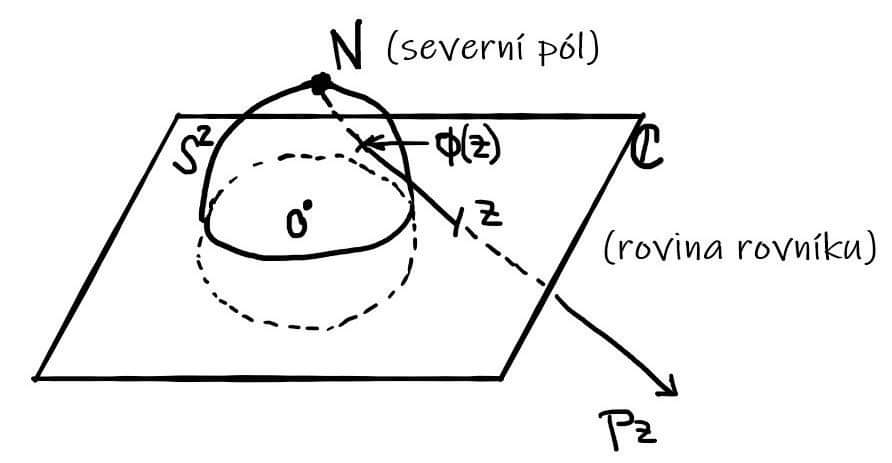
\includegraphics[width=\textwidth]{images/obrazek1.jpeg}$ 
    Položme $\phi(\infty):=N$. Pro $z\in\Comp  $ je $\{\phi(z)\}=(S\setminus \{N\})\cap p_z$, kde $p_z$ je polopřímka z $N$ procházející bodem $z\in\Comp  $. Potom $\phi:\Sp\xrightarrow[]{na}S^2$ je bijekce.
    \begin{excercise}
    \mbox{}
     \begin{itemize}
        \item[\textbullet] $\phi(z):=\left(\frac{2x}{x^2+y^2+1},\frac{2y}{x^2+y^2+1},\frac{x^2+y^2-1}{x^2+y^2+1}\right)$, $z=x+iy \in \Comp  $.
        \item[\textbullet] $\phi^{-1}(\alpha,\,\beta,\,\gamma):=\left(\frac{\alpha}{1-\gamma},\frac{\beta}{1-\gamma}\right)$, pro  $(\alpha,\,\beta,\,\gamma)\in S^2\setminus \{N\}$
     \end{itemize}
    \end{excercise}
    \item Položme $\varrho(z,\,w):=|\phi(z)-\phi(w)|$, $z,\,w\in\Sp$, kde $|\cdot|_S$ je eukleidovská norma  v $\Real ^3$. Potom $\phi$ je izometrie $(\Sp,\varrho)$ na $S^2$.
     
    \item Platí \cref{eqn:7.4.*}. Skutečně, z předchozího bodu a z cvičení máme: $\varrho(z_n,\,z_0)\rightarrow0\Leftrightarrow\phi(z_n)\rightarrow\phi(z_0)\Leftrightarrow z_n\rightarrow z_0$ v $\Sp$, protože $\phi$ i $\phi^{-1}$ jsou spojité.
    
     \item 
     Nechť $z_n\in \Comp  $ a $z_n\rightarrow \infty$. Potom $|z_n|\rightarrow+\infty$, $\phi(z_n)\in S^2$, proto  $\phi_3(z_n)\rightarrow 1$. Odtud $\phi(z_n)\rightarrow N:=(0,\,0,\,1)$
     
     \item
     Nechť $(\alpha_n,\,\beta_n,\,\gamma_n)\in S^2\setminus\{N\}$ a $(\alpha_n,\,\beta_n,\,\gamma_n)\overset{n\to\infty}{\longrightarrow} N$. Potom
     $|\phi^{-1}(\alpha_n,\,\beta_n,\,\gamma_n)|^2=\frac{1-\gamma_n^2}{(1-\gamma_n)^2}=\frac{1+\gamma_n}{1-\gamma_n}\rightarrow+\infty$. Tudíž $\phi^{-1}(\alpha_n,\,\beta_n,\,\gamma_n)\rightarrow\infty.$
\end{itemize}
\end{properties}
